\documentclass{article}

\usepackage{amsmath, amsthm, amssymb, amsfonts}
\usepackage{thmtools}
\usepackage{graphicx}
\usepackage{setspace}
\usepackage{geometry}
\usepackage{float}
\usepackage{hyperref}
\usepackage[utf8]{inputenc}
\usepackage[english]{babel}
\usepackage{framed}
\usepackage[dvipsnames]{xcolor}
\usepackage{tcolorbox}

\colorlet{LightGray}{White!90!Periwinkle}
\colorlet{LightOrange}{Orange!15}
\colorlet{LightGreen}{Green!15}
\colorlet{LightBlue}{Cyan!15}

\newcommand{\HRule}[1]{\rule{\linewidth}{#1}}

\declaretheoremstyle[name=Theorem,]{thmsty}
\declaretheorem[style=thmsty,numberwithin=section]{theorem}
\tcolorboxenvironment{theorem}{colback=LightGray}

\declaretheoremstyle[name=Proposition,]{prosty}
\declaretheorem[style=prosty,numberlike=theorem]{proposition}
\tcolorboxenvironment{proposition}{colback=LightOrange}

\declaretheoremstyle[name=Principle,]{prcpsty}
\declaretheorem[style=prcpsty,numberlike=theorem]{principle}
\tcolorboxenvironment{principle}{colback=LightGreen}

\declaretheoremstyle[
    name=Definition,
    headfont=\bfseries, % bold heading
    notebraces={(}{)},  % format for the heading
    headpunct={:},      % punctuation after the heading
    postheadspace=1em,  % space after the heading
    spaceabove=\baselineskip,
    spacebelow=\baselineskip,
]{defsty}
\declaretheorem[style=defsty,numberlike=theorem]{definition}
\tcolorboxenvironment{definition}{colback=LightBlue}


\setstretch{1.2}
\geometry{
    textheight=9in,
    textwidth=5.5in,
    top=1in,
    headheight=12pt,
    headsep=25pt,
    footskip=30pt
}

% ------------------------------------------------------------------------------

\begin{document}

% ------------------------------------------------------------------------------
% Cover Page and ToC
% ------------------------------------------------------------------------------

\title{ \normalsize \textsc{}
		\\ [2.0cm]
		\HRule{1.5pt} \\
		\LARGE \textbf{\uppercase{Optimal Control}
		\HRule{2.0pt} \\ [0.6cm] \LARGE{MAE 546 : Fall 2024} \vspace*{10\baselineskip}}
		}
\date{}
\author{\textbf{Nathaniel Chen} \\ 
		Ryne Beeson \\
		Andlinger 017 \\
		9:30-10:50 AM}

\maketitle
\newpage

\tableofcontents
\newpage

% ------------------------------------------------------------------------------

\section{Course Overview}
hi
\section{Definitions}
\begin{enumerate}
    \item Metric Space
    \item Inner Product Induced Metric
    \item Topology
    \item Open \& Closed Sets
    \item Open \& Closed Balls
    \item Metric Topology
    \item Set Closure
    \item Set Interior
    \item Open Neighborhood
\end{enumerate}

\begin{definition}{Metric Space}

    Let
    \begin{itemize}
        \item $(M,d)$: a metric space
        \item $M$: a set with topology induced by $d$
        \item $d: M \times M -> [0, \infty)$
    \end{itemize}
    Then
    \begin{enumerate}
        \item d(x,y) = d(y,x) \forall x,y \in M \hfill\text{Symmetric}
        \item d(x,x) = 0 \forall x \in M
        \item d(x,y) > 0, \forall x,y \in M, x \neq y \hfill\text{Non-Negative}
        \item d(x,y) \leq d(x,z) + d(z,y) \forall x,y,z \in M\hfill{Triangle Inequality}
    \end{enumerate}

\end{definition}

\begin{definition}{Inner Product Induced Metric}

    Let
    \begin{itemize}
        \item $(M, \langle \cdot, \cdot \rangle)$: an inner product space
        \item $M$: a vector space
        \item $\langle \cdot, \cdot \rangle$: an inner product
    \end{itemize}
    This induces the metric
    \begin{equation}
        d(x,y) = |x-y| \equiv \langle x-y, x-y \rangle^{1/2}, \forall x,y \in M
    \end{equation}

\end{definition}

\begin{definition}{Topology}
    
\end{definition}

\begin{definition}{Open \& Closed Sets}
    
\end{definition}

\begin{definition}{Open \& Closed Balls}
    
\end{definition}

\begin{definition}{Metric Topology}
    
\end{definition}

\begin{definition}{Set Closure}
    
\end{definition}

\begin{definition}{Set Interior}
    
\end{definition}

\begin{definition}{Open Neighborhood}
    
\end{definition}
\section{Examples}

\begin{theorem}
    This is a theorem.
\end{theorem}

\begin{proposition}
    This is a proposition.
\end{proposition}

\begin{principle}
    This is a principle.
\end{principle}

% Maybe I need to add one more part: Examples.
% Set style and colour later.

\subsection{Pictures}

\begin{figure}[htbp]
    \center
    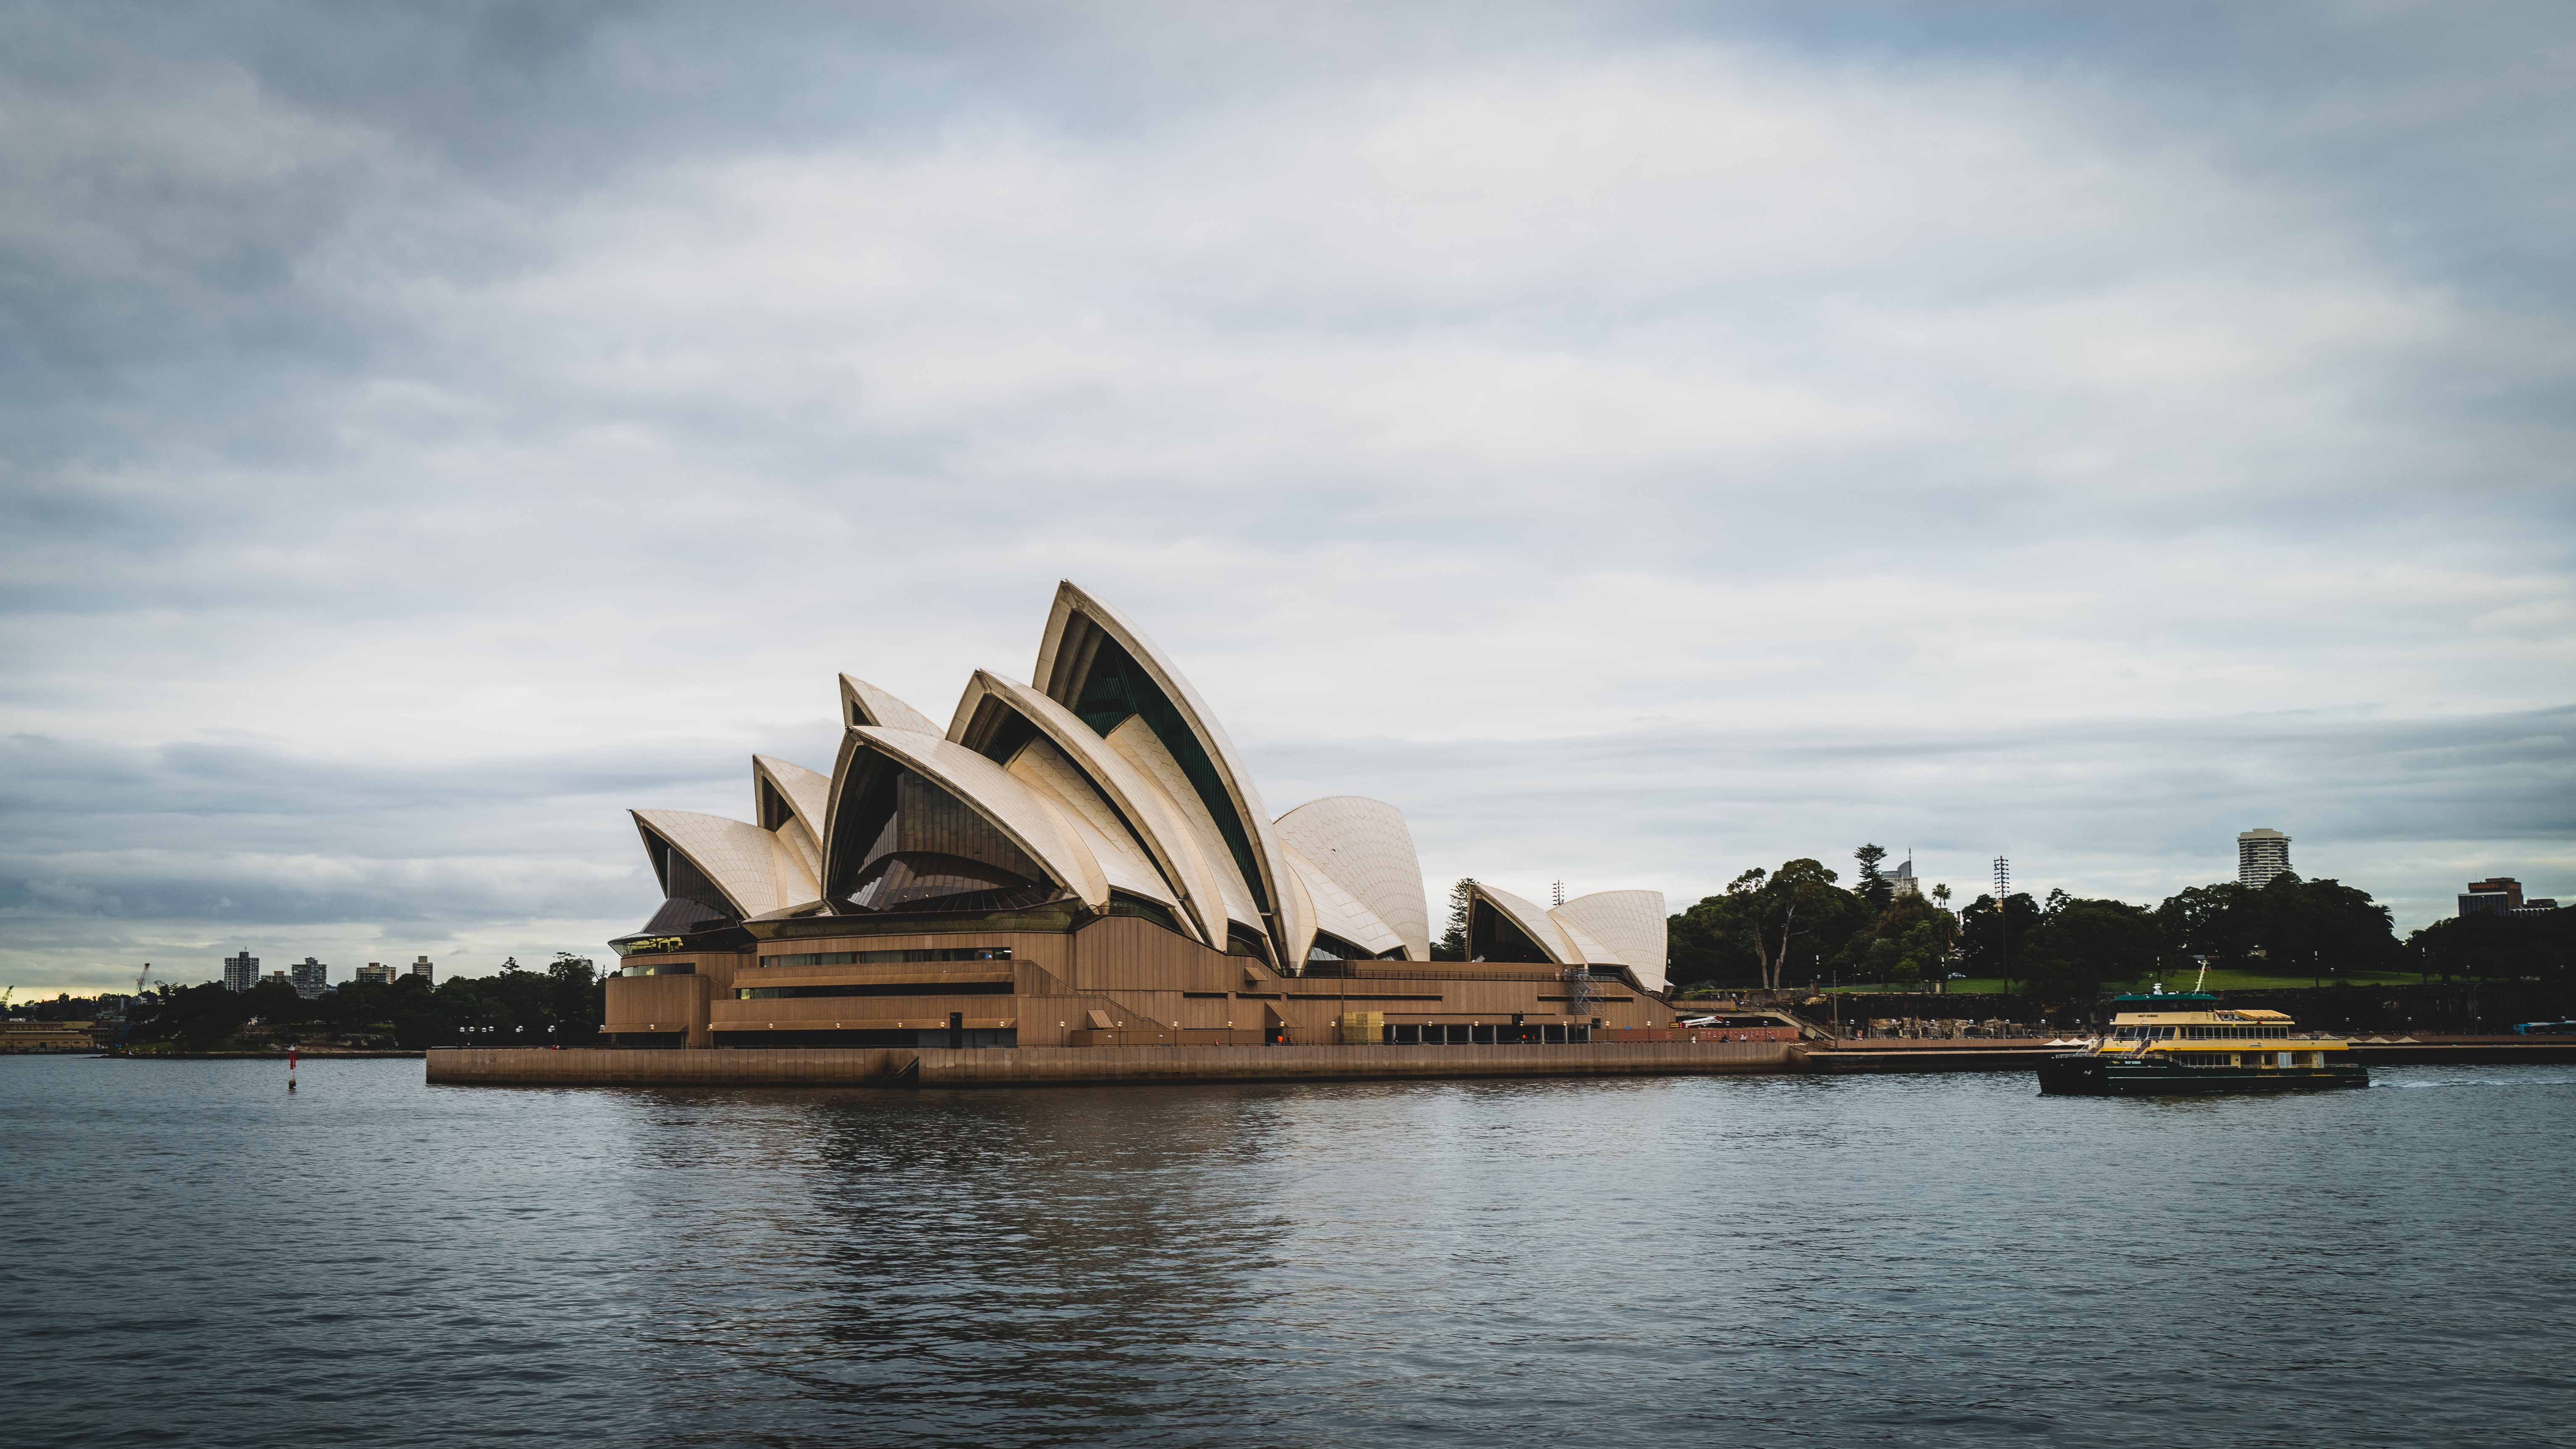
\includegraphics[scale=0.06]{img/photo.jpg}
    \caption{Sydney, NSW}
\end{figure}

\subsection{Citation}

This is a citation\cite{Eg}.

\newpage

% ------------------------------------------------------------------------------
% Reference and Cited Works
% ------------------------------------------------------------------------------

\bibliographystyle{IEEEtran}
\bibliography{References.bib}

% ------------------------------------------------------------------------------

\end{document}
